\documentclass[preprint,12pt]{elsarticle}
\usepackage[T1]{fontenc}
\usepackage[utf8]{inputenc}
\usepackage{amsmath,amssymb}
\usepackage{graphicx}
\usepackage{booktabs}
\usepackage{array}
\usepackage{multirow}
\usepackage{siunitx}
\usepackage{tabularx}
\usepackage{xurl}
\usepackage[hidelinks]{hyperref}
\usepackage{xcolor}
\usepackage{tikz}
\usepackage{placeins}
\usetikzlibrary{arrows.meta,positioning,shapes.geometric,fit}

\journal{Biomedical Signal Processing and Control}

\hypersetup{
  pdftitle={Signal-Quality Admissibility for Sensorimotor Rhythm Neurofeedback: Beyond High-Beta Inhibition},
  pdfauthor={Suzana Cescon de Souza and Antonio Pereira Jr}
}

\newcommand{\doiurl}[1]{\href{https://doi.org/#1}{\nolinkurl{#1}}}

% Reduces avoidable overfull lines in dense Elsevier preprint text.
\setlength{\emergencystretch}{2em}

\begin{document}

\begin{frontmatter}

\title{Signal-Quality Admissibility for Sensorimotor Rhythm Neurofeedback: Beyond High-Beta Inhibition}

\author[1]{Suzana Cescon de Souza}
\author[1]{\texorpdfstring{Antonio Pereira Jr\corref{cor1}}{Antonio Pereira}}
\cortext[cor1]{Corresponding author: \texttt{apereira@ufpa.br}}

\affiliation[1]{
organization={Signal Processing Laboratory, Institute of Technology, Postgraduate Program in Electrical Engineering, Federal University of Par\'a},
city={Bel\'em},
state={Par\'a},
country={Brazil}
}

\begin{abstract}
Sensorimotor rhythm (SMR) neurofeedback commonly rewards 12--15 Hz sensorimotor activity while inhibiting high-beta activity. The inhibit band is often treated as part of the training rule, although scalp high-beta power is a mixed physiological and technical measure. We tested whether high-beta inhibition functions better as a signal-quality screen than as a specific neural control index. Using public high-density SMR-BCI datasets, we evaluated offline candidate feedback windows under three rules: SMR-only reward, SMR plus high-beta inhibition, and a multicomponent neurofeedback signal-quality index (NF-SQI). NF-SQI combined high beta, broadband power, 35--45 Hz noise-floor power, transient amplitude, and channel consistency. In the harmonized SMR-SNR analysis across ds004447, ds004444, and ds004446, high-beta inhibition alone blocked only 29.2--42.3\% of rule-defined quality-flagged SMR candidates, whereas broadband/noise-floor criteria blocked 63.4--65.6\%, and exclusively high-beta contamination accounted for just 4.5\% of flagged candidates. In leave-one-subject-out prediction of rule-defined signal-quality flags, broadband/noise-floor predictors outperformed high beta by +0.100 to +0.191 AUC, and adding high beta to broadband/noise-floor predictors did not materially improve AUC; SMR-power sensitivity analyses reproduced the same ordering. Because the full NF-SQI gate applies exactly the constraints that define a quality flag, it removes the flagged candidates by construction while retaining the clean Gate A candidates as admissible feedback, corresponding to 38.0--52.2\% of SMR-only candidates, 6.5--9.0\% of all task-compatible windows, and 7.8--10.9 retained windows per minute. A raw-window pseudo-online replay of the gate on the source recordings reproduced the offline Gate A and Gate B counts exactly in all three datasets and the Gate C counts either exactly or to within a single window, at a mean compute latency near 1 ms per 1 s window, establishing that the rule is reproducible in a streaming loop. These results support interpreting high-beta inhibition as a useful but incomplete signal-quality proxy, and NF-SQI as an explicit, deployable admissibility rule that separates target-band reward from signal-quality control.
\end{abstract}

\begin{keyword}
neurofeedback \sep sensorimotor rhythm \sep brain-computer interface \sep EEG signal quality \sep high beta \sep artifact control \sep admissibility gating
\end{keyword}

\end{frontmatter}

\section{Introduction}

Sensorimotor rhythm (SMR) neurofeedback uses ongoing electroencephalography (EEG) to reinforce sensorimotor-band modulation in the 12--15 Hz range over central scalp regions. This target band originates from the classical SMR neurofeedback literature, which treats low-beta reinforcement as an operant mechanism for sensorimotor regulation \citep{StermanEgner2006,EgnerGruzelier2004}. SMR-based brain-computer interfaces and neurofeedback systems are grounded in event-related synchronization and desynchronization phenomena of sensorimotor rhythms \citep{Pfurtscheller1999ERD,Wolpaw2002BCI}. Large open datasets now make it possible to evaluate SMR-BCI signal-processing assumptions across subjects and sessions \citep{Stieger2021SMRBCI,Iwama2023HDEEG}. In these systems, performance is not only determined by whether the target frequency is present. It also depends on whether the target estimate is obtained from an admissible signal state.

Many SMR neurofeedback protocols use compound feedback rules: increase SMR while inhibiting non-target bands. A representative protocol trained participants to increase SMR at 12--15 Hz while inhibiting theta and high beta at 21--30 Hz across C3, Cz, and C4 \citep{Dessy2020Train}. Such designs embed an important engineering assumption. The high-beta inhibit channel is expected to protect the feedback loop from undesirable states. However, high beta is not a mechanistically pure scalp-EEG variable. Scalp muscle activity can obscure or mimic EEG beta rhythms across the scalp, and direct paralysis recordings show that EEG power above 20 Hz is strongly contaminated by EMG \citep{Goncharova2003EMG,Whitham2007ScalpEMG}. High-frequency EEG activity therefore overlaps with the spectral range of muscle activity, and muscle artifacts can dominate scalp high-frequency measurements \citep{Muthukumaraswamy2013Muscle}.

This creates a measurement problem for neurofeedback. If high-beta inhibition is interpreted as a neural mechanism, the same band-power change may be overread as evidence of sensorimotor regulation. This concern is aligned with broader debates about neurofeedback specificity, control beliefs, and mechanistic interpretation \citep{Thibault2016SelfRegulating,Witte2013ControlBeliefs}. If high-beta inhibition is interpreted as a signal-quality safeguard, the question changes: does the inhibit channel prevent an SMR reward rule from accepting contaminated windows? This framing connects neurofeedback to biomedical signal-quality control rather than to a single-band neural mechanism. It also aligns with modern EEG processing practice, in which rejection or correction policies are evaluated as part of the measurement pipeline \citep{Jas2017Autoreject,BigdelyShamlo2015PREP,Delorme2004EEGLAB,Gramfort2013MNE}.

We introduce a neurofeedback signal-quality index (NF-SQI) that treats high-beta inhibition as one admissibility feature among several. The objective is not to infer whether high beta is neural, muscular, attentional, or arousal-related in each window. The objective is to quantify whether high beta improves the rejection of false-admissible SMR windows and whether a multicomponent quality gate outperforms conventional high-beta-only inhibition. The primary analysis uses OpenNeuro ds004447 and companion replication analyses use ds004444 and ds004446 from the same high-density SMR-BCI collection \citep{Iwama2023HDEEG,OpenNeuroDS004444,OpenNeuroDS004446,OpenNeuroDS004447}. Across datasets, we compare three virtual feedback gates: an SMR-only gate, an SMR plus high-beta-inhibit gate, and a full NF-SQI gate. The central result is that high beta blocks a real but mostly overlapping subset of false-admissible candidate windows. The strongest engineering solution is therefore not a stronger high-beta interpretation, but an explicit multicomponent signal-quality framework.

\section{Methods}

\subsection{Dataset}

We analyzed compatible public OpenNeuro BMI-HDEEG datasets from the high-density SMR-BCI collection described by \citep{Iwama2023HDEEG}. The primary reproduction dataset was ds004447, The BMI-HDEEG dataset 3 \citep{OpenNeuroDS004447}. Companion replication analyses used ds004444, The BMI-HDEEG dataset 1 \citep{OpenNeuroDS004444}, and ds004446, The BMI-HDEEG dataset 2 \citep{OpenNeuroDS004446}. Dataset ds004448 was inventoried but not analyzed because the available local event structure contained only trial-start markers and did not support the same rest/task-compatible thresholding path. The analyzed subsets contained 22 subjects and 44 EDF files in ds004447, 30 subjects and 60 EDF files in ds004444, and 5 subjects and 10 EDF files in ds004446. The raw recordings were sampled at 1000 Hz. No online reward or feedback event markers were available; all reward rules below are therefore virtual gates applied offline to task windows. This design tests signal-quality admissibility of candidate feedback states.

The primary sensorimotor channels were E36, E104, and E128, following the dataset helper-code equivalents for C3/C4/Cz-like central scalp sites. Analyses were performed on the combined central-channel representation and repeated in channel-sensitivity checks.

\begin{table}[htbp]
\centering
\small
\caption{Dataset and primary analysis settings.}
\label{tab:dataset}
\begin{tabularx}{\textwidth}{@{}>{\raggedright\arraybackslash}p{0.34\textwidth}
>{\raggedright\arraybackslash}X@{}}
\toprule
Component & Specification \\
\midrule
Datasets analyzed & ds004447 primary; ds004444 and ds004446 replication \\
Dataset inventoried but skipped & ds004448 \\
Subjects analyzed & 22, 30, and 5 by dataset \\
EDF files analyzed & 44, 60, and 10 by dataset \\
Sampling rate & 1000 Hz \\
Reward markers & not present in event sidecars \\
Sensorimotor channels & E36, E104, E128 \\
Primary window & 1 s, 50\% overlap \\
Sensitivity windows & 0.5 s and 2 s, 50\% overlap \\
SMR band & 12--15 Hz \\
High-beta band & 20--30 Hz \\
Noise-floor band & 35--45 Hz \\
Broadband non-target power & 4--45 Hz excluding SMR and high beta \\
\bottomrule
\end{tabularx}
\end{table}


\subsection{Preprocessing and spectral estimation}

All EDF files were processed with the same deterministic windowing and spectral-estimation pipeline before gate construction. Signals were analyzed at the native 1000 Hz sampling rate; no resampling was applied. The NF-SQI code did not apply rereferencing, explicit temporal filtering, manual artifact rejection, independent-component rejection, or visual cleaning before the virtual gates. The analysis therefore tests whether computable gate features can screen candidate windows under the measurement conditions available to an online system. The only implicit detrending step was the default constant detrending applied by \texttt{scipy.signal.welch} during spectral estimation.

For each 1 s task window, the central signal was formed by averaging E36, E104, and E128 before spectral estimation. Power spectral density was estimated using Welch's method with the default Hann window and \texttt{nperseg} equal to the window length. At the native 1000 Hz sampling rate and 1 s primary window, the resulting frequency resolution was 1 Hz. Band power was obtained by trapezoidal integration of the spectral density over inclusive frequency masks. The frequency bands were SMR, 12--15 Hz; high beta, 20--30 Hz; broadband non-target activity, 4--45 Hz excluding the SMR and high-beta bands; and high-frequency noise floor, 35--45 Hz. Per-channel powers were used separately for the channel-inconsistency feature.

Primary thresholds were fit from rest-baseline distributions within the corresponding subject and session. The primary cutoff was the 75th percentile for SMR evidence, high beta, broadband, noise floor, and channel inconsistency, and the 90th percentile for transient amplitude. MAD thresholds and task-baseline thresholds were used only as sensitivity analyses. In predictive modeling, scaling and model fitting were performed within each training fold, and held-out-subject information was excluded from the fitted scaler and classifier.

\subsection{Window-level signal-quality features}

For each task window, we computed SMR power, SMR signal-to-noise ratio (SNR), high-beta power, broadband non-target power, high-frequency noise-floor power, transient-amplitude score, and channel-inconsistency score. SMR SNR was computed as target-band power relative to non-target spectral activity. Broadband non-target power summarized 4--45 Hz activity after excluding the SMR and high-beta bands. The high-frequency noise floor was defined as 35--45 Hz activity.

Transient score was the maximum absolute amplitude within the native window. Channel inconsistency was defined as the standard deviation of standardized power metrics across E36, E104, and E128 within the same window. Standardization was performed within subject, session, and channel using rest-baseline distributions. A median absolute deviation version was computed as a robust sensitivity metric.

\subsection{Engineering formulation}

Let \(y_w(t)\) denote the observed EEG in window \(w\). The measurement model is
\begin{equation}
    y_w(t) = s_{\mathrm{SMR},w}(t) + c_{\mathrm{HB},w}(t) + c_{\mathrm{BB},w}(t) + c_{\mathrm{TR},w}(t) + \epsilon_w(t),
\end{equation}
where \(s_{\mathrm{SMR},w}\) is the target SMR component, \(c_{\mathrm{HB},w}\) is high-beta activity, \(c_{\mathrm{BB},w}\) is broadband or high-frequency contamination, \(c_{\mathrm{TR},w}\) denotes transient high-amplitude contamination, and \(\epsilon_w\) is residual noise. The admissibility problem is to accept a candidate feedback window only when target evidence is present and contamination indicators remain below predefined limits.

The SMR evidence variable is denoted by \(\Gamma_w\). In the primary harmonized analysis, \(\Gamma_w\) was SMR SNR in ds004447, ds004444, and ds004446. SMR power was evaluated as a sensitivity target scalar and reproduced the same ordering of gate performance.

The SMR-only admissibility set is
\begin{equation}
    \mathcal{A}_{\mathrm{SMR}} = \{w: \Gamma_w > \theta_{\mathrm{SMR}}\}.
\end{equation}
The high-beta-inhibited set is
\begin{equation}
    \mathcal{A}_{\mathrm{HB}} = \{w: \Gamma_w > \theta_{\mathrm{SMR}},\; \mathrm{HB}_w < \theta_{\mathrm{HB}}\}.
\end{equation}
The full NF-SQI admissibility set is
\begin{equation}
\begin{split}
    \mathcal{A}_{\mathrm{SQI}} = \{w: &\; \Gamma_w > \theta_{\mathrm{SMR}},\; \mathrm{HB}_w < \theta_{\mathrm{HB}},\; \mathrm{BB}_w < \theta_{\mathrm{BB}}, \\
    &\; \mathrm{NF}_w < \theta_{\mathrm{NF}},\; \mathrm{TR}_w < \theta_{\mathrm{TR}},\; \mathrm{CI}_w < \theta_{\mathrm{CI}}\},
\end{split}
\end{equation}
where BB is broadband non-target power, NF is high-frequency noise-floor power, TR is transient-amplitude score, and CI is channel inconsistency.

\begin{figure}[htbp]
\centering
\resizebox{0.98\textwidth}{!}{%
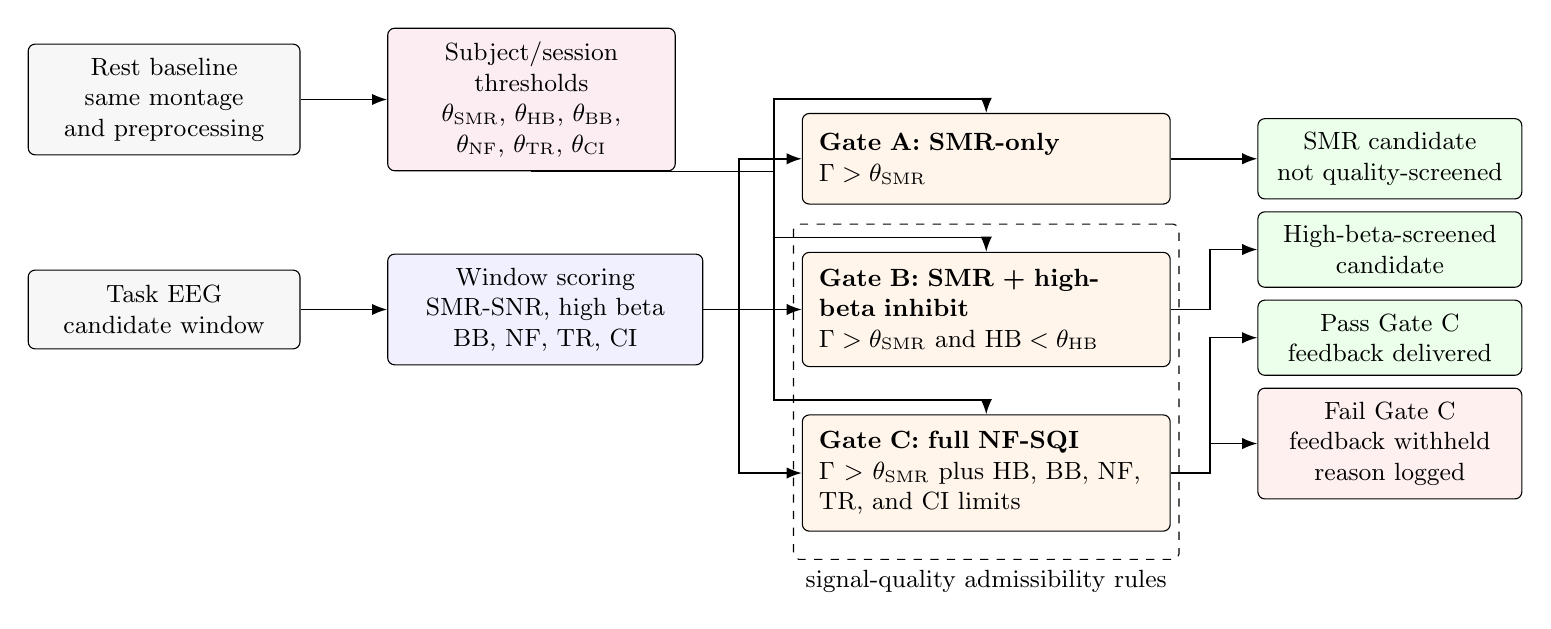
\begin{tikzpicture}[
    >=Latex,
    font=\small,
    node distance=0.95cm and 1.10cm,
    box/.style={draw, rounded corners=2.5pt, align=center, minimum height=1.00cm, text width=3.10cm, inner sep=5pt, fill=gray!6},
    feature/.style={draw, rounded corners=2.5pt, align=center, minimum height=1.00cm, text width=3.65cm, inner sep=5pt, fill=blue!6},
    calib/.style={draw, rounded corners=2.5pt, align=center, minimum height=0.95cm, text width=3.30cm, inner sep=5pt, fill=purple!7},
    gate/.style={draw, rounded corners=2.5pt, align=left, minimum height=1.15cm, text width=4.25cm, inner sep=6pt, fill=orange!8},
    pass/.style={draw, rounded corners=2.5pt, align=center, minimum height=0.90cm, text width=3.00cm, inner sep=5pt, fill=green!8},
    fail/.style={draw, rounded corners=2.5pt, align=center, minimum height=0.90cm, text width=3.00cm, inner sep=5pt, fill=red!6},
    arrow/.style={->, line width=0.55pt}
]
\node[box] (rest) {Rest baseline\\same montage and preprocessing};
\node[calib, right=of rest] (thresholds) {Subject/session\\thresholds\\$\theta_{\mathrm{SMR}}$, $\theta_{\mathrm{HB}}$, $\theta_{\mathrm{BB}}$, $\theta_{\mathrm{NF}}$, $\theta_{\mathrm{TR}}$, $\theta_{\mathrm{CI}}$};
\node[box, below=1.45cm of rest] (eeg) {Task EEG\\candidate window};
\node[feature, right=of eeg] (features) {Window scoring\\SMR-SNR, high beta\\BB, NF, TR, CI};
\node[gate, right=1.25cm of features] (gateb) {\textbf{Gate B: SMR + high-beta inhibit}\\$\Gamma > \theta_{\mathrm{SMR}}$ and $\mathrm{HB}<\theta_{\mathrm{HB}}$};
\node[gate, above=0.6cm of gateb] (gatea) {\textbf{Gate A: SMR-only}\\$\Gamma > \theta_{\mathrm{SMR}}$};
\node[gate, below=0.6cm of gateb] (gatec) {\textbf{Gate C: full NF-SQI}\\$\Gamma > \theta_{\mathrm{SMR}}$ plus HB, BB, NF, TR, and CI limits};
\coordinate (busT) at ([xshift=0.9cm]features.east);
\coordinate (gateaAbove) at ([yshift=0.18cm]gatea.north);
\coordinate (gatebAbove) at ([yshift=0.18cm]gateb.north);
\coordinate (gatecAbove) at ([yshift=0.18cm]gatec.north);
\node[pass, right=of gatea] (outa) {SMR candidate\\not quality-screened};
\node[pass, below=0.15cm of outa] (outb) {High-beta-screened\\candidate};
\node[pass, below=0.15cm of outb] (reward) {Pass Gate C\\feedback delivered};
\node[fail, below=0.15cm of reward] (withhold) {Fail Gate C\\feedback withheld\\reason logged};
\draw[arrow] (rest) -- (thresholds);
\draw[arrow] (thresholds.south) -- (thresholds.south -| busT) -- (gateaAbove -| busT) -- (gateaAbove) -- (gatea.north);
\draw[arrow] (thresholds.south) -- (thresholds.south -| busT) -- (gatebAbove -| busT) -- (gatebAbove) -- (gateb.north);
\draw[arrow] (thresholds.south) -- (thresholds.south -| busT) -- (gatecAbove -| busT) -- (gatecAbove) -- (gatec.north);
\draw[arrow] (eeg) -- (features);
\draw[arrow] (features.east) -- ++(0.45,0) |- (gatea.west);
\draw[arrow] (features.east) -- ++(0.45,0) -- (gateb.west);
\draw[arrow] (features.east) -- ++(0.45,0) |- (gatec.west);
\draw[arrow] (gatea.east) -- ++(0.3,0) |- (outa.west);
\draw[arrow] (gateb.east) -- ++(0.5,0) |- (outb.west);
\draw[arrow] (gatec.east) -- ++(0.5,0) |- (reward.west);
\draw[arrow] (gatec.east) -- ++(0.5,0) |- (withhold.west);
\node[draw, dashed, rounded corners=2pt, fit=(gateb) (gatec), inner xsep=3pt, inner ysep=10pt,
      label={[font=\small]below:signal-quality admissibility rules}] (qualitybox) {};
\end{tikzpicture}%
}
\caption{NF-SQI admissibility workflow. Rest-baseline data are used to estimate subject- and session-specific thresholds. Each task EEG candidate window is scored for SMR evidence and signal-quality features. Gate A accepts windows using only SMR evidence, Gate B adds the conventional high-beta inhibit rule, and Gate C applies the full NF-SQI rule combining high beta, broadband/noise-floor, transient-amplitude, and channel-consistency constraints. Gate C does not eliminate feedback by definition: windows that pass both SMR and quality criteria remain admissible for feedback, whereas flagged windows are withheld and logged with rejection reasons. The primary harmonized analysis used SMR SNR as the target-evidence variable across ds004447, ds004444, and ds004446; SMR power was evaluated as a sensitivity analysis.}
\label{fig:framework}
\end{figure}

\subsection{Virtual gate definitions}

Three virtual gates were compared. Gate A accepted a window if it met the SMR evidence criterion. Gate B accepted a window if it met the SMR evidence criterion and remained below the high-beta threshold. Gate C accepted a window if it met the SMR evidence criterion and satisfied all NF-SQI quality constraints.

A quality-flagged Gate A window was defined as an SMR-only candidate window carrying at least one prespecified signal-quality flag: high beta, broadband/noise-floor, transient-amplitude, or channel-inconsistency. The blocking analysis is therefore a rule-coverage analysis: it quantifies how much of the prespecified quality-flagged SMR-candidate set is removed by each gate component. It is not presented as an external ground-truth artifact-classification benchmark. The independent comparison across feature groups is provided by the leave-one-subject-out predictive models described below.

Contamination-overlap decomposition separated clean windows, exclusively high-beta flagged windows, exclusively broadband/noise flagged windows, exclusively transient flagged windows, exclusively channel-inconsistency flagged windows, and multi-flagged windows. The main overlap percentages are subject-session means. Count-weighted denominator accounting is reported separately to clarify the number of task-compatible windows, Gate A candidates, Gate B accepted windows, and Gate C accepted windows.

\subsection{Deployment threshold policy}

For deployment, NF-SQI thresholds are intended to be subject- and session-specific. A rest baseline acquired with the same montage, sampling rate, signal units, and preprocessing as the training session is used to estimate the admissibility limits. In the reference configuration, the SMR evidence threshold, high-beta threshold, broadband threshold, noise-floor threshold, and channel-inconsistency threshold are set from the 75th percentile of the corresponding rest-baseline distribution, whereas the transient-amplitude threshold is set from the 90th percentile. During training or pseudo-online replay, a task window is first tested for SMR evidence. It is then admitted for feedback only if it remains below all signal-quality limits.

This policy separates two decisions that are often conflated in neurofeedback. The SMR threshold defines whether the target rhythm is sufficiently expressed. The NF-SQI quality thresholds define whether the window is trustworthy enough to use for reinforcement. Prospective online systems may tune these percentiles to preserve a sufficient reinforcement rate, but the default policy provides a transparent starting point for reproducing and comparing admissibility rules.

\subsection{Operating point and feedback-density metrics}

To evaluate whether the default threshold policy produced a usable reward stream, we computed the retained-window density for Gate A, Gate B, and Gate C. Feedback density was expressed as accepted windows per minute using the 1 s windows with 50\% overlap. We also swept the percentile thresholds from p50 to p95 to characterize the operating tradeoff between admissible-window yield and quality-flag blocking. The default p75/p90 configuration was treated as a prespecified conservative reference policy, not as an optimized operating point. This analysis allows the operating point to be shifted depending on whether the target application prioritizes denser feedback or stricter signal-quality admissibility.

\subsection{Real-data pseudo-online replay}
\label{sec:pseudo_online_methods}

To verify that the admissibility rule is reproducible in a streaming loop rather than only as an offline batch computation, we implemented a raw-window pseudo-online replay that drives the deployment reference implementation directly from the OpenNeuro EDF recordings. For each session, the three central channels were loaded and task samples were labelled from the events sidecar. The recording was segmented into 1 s windows at 0.5 s hop; windows composed of more than 50\% task samples formed the replay stream, and the remaining windows formed the rest-baseline calibration set, matching the offline windowing exactly. NF-SQI decision limits and the channel-inconsistency baseline were calibrated from the rest windows using the deployment calibration routine, and each task window was then scored through the same per-window evaluation function used by the online rolling-window helper. For every window we recorded the Gate A, Gate B, and Gate C decision, the rejection reasons, and the wall-clock compute latency. Counts, feedback density, and latency were aggregated per session, per subject, and pooled per dataset, and compared against the offline batch counts. This replay used the same central channels, window length, frequency bands, thresholds, and target-evidence scalar as the primary analysis, so that agreement with the batch pipeline tests the streaming implementation rather than a re-tuned rule.

\subsection{Predictive modeling and robustness}

Cross-validated models predicted prespecified signal-quality labels from candidate feature groups. Logistic regression was used deliberately as a transparent linear ablation model, not as an attempt to maximize classifier performance. The purpose was to compare whether high beta, broadband/noise-floor activity, and the full NF-SQI feature set carried discriminative information under the same leakage-controlled validation scheme.

Model A used broadband and noise-floor predictors. Model B used high beta only. Model C used broadband/noise-floor plus high beta. Model D used the full NF-SQI feature set. Classifiers were balanced logistic regression models \citep{Pedregosa2011Scikit}. Continuous predictors were standardized within cross-validation using training subjects only, and the held-out subject was transformed with the corresponding training-fitted scaler. Leave-one-subject-out grouping was used to prevent subject-level leakage and to approximate deployment on unseen participants \citep{Saeb2017UseCase}. Performance was summarized with area under the ROC curve (AUC), balanced accuracy, precision, and recall.

Robustness analyses varied thresholds, baseline source, and channel definitions. Subject influence was quantified by recomputing the high-beta blocking percentage after excluding each subject. Gate performance was also summarized across 70th, 80th, 90th percentile and MAD thresholds using rest and task baselines. Task-baseline thresholds were treated only as sensitivity analyses because primary admissibility thresholds should be fit without using the same task distribution that the gate later classifies.

\subsection{Replication and uncertainty}

The ds004447 analysis was reproduced and then tested in compatible companion datasets ds004444 and ds004446 using the same central channels, window length, frequency bands, quality constraints, target-evidence scalar, and leave-one-subject-out validation structure. The primary harmonized analysis used SMR SNR as the Gate A target scalar in all analyzed datasets. SMR power was evaluated as a sensitivity analysis. Dataset ds004448 was not forced because its local event structure did not provide a safe rest/task-compatible analysis path. Uncertainty intervals were computed by subject-level grouped bootstrap with 5000 resamples, percentile 95\% confidence intervals, and random seed 20260702. Bootstrap resampling preserved all sessions and windows within each sampled subject.

\subsection{Formal difference tests}

Formal comparisons between gate components and predictive models were performed with subject-grouped bootstrap difference tests. Each bootstrap resample preserved the subject as the sampling unit and retained all available sessions and windows within the sampled subject. For blocking analyses, the tested contrasts were broadband/noise-floor blocking minus high-beta blocking, full NF-SQI blocking minus high-beta blocking, and full NF-SQI blocking minus broadband/noise-floor blocking. For predictive models, the tested contrasts were broadband/noise-floor AUC minus high-beta AUC, full NF-SQI AUC minus high-beta AUC, and broadband/noise-floor plus high-beta AUC minus broadband/noise-floor AUC.

For each contrast, we report the paired bootstrap difference, percentile 95\% confidence interval, and two-sided bootstrap \(p\)-value from 5000 resamples. Bootstrap \(p\)-values equal to zero are reported as \(p<0.001\). These tests evaluate paired differences under the same subject-grouped resampling structure used for the primary uncertainty intervals.

\section{Results}


\subsection{Signal-level examples}

Representative clean and contaminated SMR-candidate windows show the signal structure targeted by the admissibility framework (Fig.~\ref{fig:example_windows}). Both examples are candidate SMR windows at the target-selection stage, but the contaminated example expresses stronger non-target spectral structure in the high-beta and high-frequency noise-floor ranges. The full-window analyses below quantify this distinction across all subject-session contrasts.

\begin{figure}[htbp]
\centering

\includegraphics[width=0.94\textwidth]{nf_sqi_example_windows_psd.pdf}
\caption{Representative clean and contaminated SMR-candidate windows. Panels A and C show 1-s central-channel time-domain traces. Panels B and D show the corresponding spectra, with the SMR, high-beta, and noise-floor bands shaded. The clean candidate was extracted from sub-021, session 19, at 100.0 s. The contaminated candidate was extracted from sub-019, session 19, at 36.5 s and carried broadband and noise-floor contamination flags.}
\label{fig:example_windows}
\end{figure}

\subsection{Candidate-window composition}

Across subject-session contrasts, 53.5\% of SMR-only candidate windows were clean and 46.5\% carried at least one contamination flag. Exclusive high-beta contamination accounted for 4.5\% of SMR candidates. Exclusive broadband/noise contamination accounted for 15.2\%, exclusive channel-inconsistency contamination for 9.0\%, exclusive transient contamination for 0.2\%, and multi-contamination for 17.7\% (Table~\ref{tab:overlap}; Fig.~\ref{fig:overlap_pie}). These values are subject-session means and therefore are not identical to count-weighted denominator percentages.

\begin{table}[htbp]
\centering
\caption{Contamination-overlap decomposition of SMR-only candidate windows. Values are mean proportions across subject-session contrasts.}
\label{tab:overlap}
\begin{tabular}{lS[table-format=2.1]}
\toprule
Candidate-window class & {Proportion (\%)} \\
\midrule
Clean & 53.5 \\
Exclusively high-beta contaminated & 4.5 \\
Exclusively broadband/noise contaminated & 15.2 \\
Exclusively channel-inconsistency contaminated & 9.0 \\
Exclusively transient contaminated & 0.2 \\
Multi-contaminated & 17.7 \\
\bottomrule
\end{tabular}
\end{table}

\begin{table}[htbp]
\centering
\footnotesize
\caption{Count-weighted denominator accounting for 1 s task windows. Gate A, Gate B, and Gate C percentages are relative to all task-compatible windows. Clean and quality-flagged percentages are relative to Gate A candidates. Blocking percentages are relative to quality-flagged Gate A candidates.}
\label{tab:denominator_accounting}
\resizebox{\textwidth}{!}{%
\begin{tabular}{lrrrrrrrrrr}
\toprule
Dataset & EDF & Subjects & Task windows & Gate A & Clean & Quality flagged & Gate B & Gate C & HB blocks & Full blocks \\
\midrule
ds004447 & 44 & 22 & 5218 & 905 (17.3\%) & 472 (52.2\%) & 433 (47.8\%) & 779 (14.9\%) & 472 (9.0\%) & 126 (29.1\%) & 433 (100.0\%) \\
ds004444 & 60 & 30 & 14400 & 2455 (17.0\%) & 933 (38.0\%) & 1522 (62.0\%) & 1811 (12.6\%) & 933 (6.5\%) & 644 (42.3\%) & 1522 (100.0\%) \\
ds004446 & 10 & 5 & 2800 & 451 (16.1\%) & 215 (47.7\%) & 236 (52.3\%) & 355 (12.7\%) & 215 (7.7\%) & 96 (40.7\%) & 236 (100.0\%) \\
\bottomrule
\end{tabular}%
}
\end{table}

By construction, quality-flagged Gate A windows equal Gate A candidates minus clean Gate A candidates, and full NF-SQI blocks equal Gate A candidates minus Gate C accepted windows. Gate C therefore should not be read as blocking all candidate feedback. It retained the clean SMR candidates: 472 windows in ds004447, 933 in ds004444, and 215 in ds004446. These retained windows corresponded to 52.2\%, 38.0\%, and 47.7\% of Gate A candidates, respectively, and to 9.0\%, 6.5\%, and 7.7\% of all task-compatible windows. Thus, the full NF-SQI rule converts a larger SMR-only candidate pool into a smaller set of admissible feedback states rather than eliminating feedback entirely.

\subsection{Operating tradeoff and feedback density}

The default p75/p90 policy produced a conservative but nonzero feedback stream. Gate C retained 9.05\%, 6.48\%, and 7.68\% of task-compatible windows in ds004447, ds004444, and ds004446, respectively (472/5218, 933/14400, and 215/2800 windows; consistent with Table~\ref{tab:denominator_accounting}). Expressed as replay density for 1 s windows with 50\% overlap, this corresponded to 10.85, 7.77, and 9.21 retained windows per minute (Table~\ref{tab:feedback_density}). Gate C therefore reduced feedback density relative to Gate A and Gate B, but it did not eliminate feedback.

Sweeping the percentile thresholds from p50 to p95 showed the expected yield--quality tradeoff. Less stringent settings increased Gate A yield but admitted more quality-flagged windows; more stringent settings reduced both contamination and retained-window density. The p75/p90 setting should therefore be interpreted as a reproducible conservative reference policy rather than an optimized operating point. In prospective online systems, this operating point can be shifted to match the required balance between feedback density and signal-quality admissibility.

\begin{table}[htbp]
\centering
\small
\caption{Feedback density under the default p75/p90 threshold policy. Gate yields are percentages of all task-compatible windows, recomputed directly from the Gate C counts in Table~\ref{tab:denominator_accounting}. Retained windows per minute were computed for Gate C using 1 s windows with 50\% overlap (hop 0.5 s).}
\label{tab:feedback_density}
\begin{tabular}{lrrrr}
\toprule
Dataset & Gate A yield (\%) & Gate B yield (\%) & Gate C yield (\%) & Gate C windows/min \\
\midrule
ds004447 & 17.34 & 14.93 & 9.05 & 10.85 \\
ds004444 & 17.05 & 12.58 & 6.48 & 7.77 \\
ds004446 & 16.11 & 12.68 & 7.68 & 9.21 \\
\bottomrule
\end{tabular}
\end{table}

\begin{figure}[htbp]
\centering
\includegraphics[width=0.86\textwidth]{nfsqi_operating_tradeoff.pdf}
\caption{Operating tradeoff between retained-window density and signal-quality admissibility. Threshold percentiles were swept from p50 to p95. The default p75/p90 setting provides a conservative reference policy: it retains a nonzero Gate C feedback stream while reducing the quality-flagged fraction of candidate windows.}
\label{fig:operating_tradeoff}
\end{figure}

\begin{figure}[htbp]
\centering

\includegraphics[width=0.92\textwidth]{nf_sqi_contamination_overlap_pie.pdf}
\caption{Composition of SMR-only candidate feedback windows. The high-beta-only fraction is small relative to broadband/noise, channel-inconsistency, and multi-contaminated classes.}
\label{fig:overlap_pie}
\end{figure}

\subsection{False-admissible blocking}

Within the rule-defined quality-flagged Gate A set for the primary dataset (ds004447), the individual quality criteria covered different and largely complementary portions of the flagged windows: high-beta inhibition alone blocked only 29.2\% of the flagged SMR-only candidates, whereas broadband/noise-floor criteria blocked 65.6\%, channel inconsistency blocked 47.9\%, and transient-amplitude thresholding blocked 4.1\% (Table~\ref{tab:blocking}; Fig.~\ref{fig:blocking}). Across the two companion datasets, high-beta blocking ranged from 40.9\% to 42.3\% and broadband/noise-floor blocking ranged from 63.4\% to 64.2\% (Section~3.6). The full NF-SQI rule blocks 100.0\% of the flagged set, but this value is a definitional identity rather than an empirical performance estimate: because a window is defined as quality-flagged precisely when it violates at least one NF-SQI constraint, the gate that enforces all of those constraints necessarily excludes the entire flagged set. We therefore report the full-gate value as an identity and base inference on the component-wise coverage above and on the leave-one-subject-out predictive comparison below, neither of which is circular. Crucially, the identity does not mean that Gate C blocked all reward candidates: Gate C retained the clean Gate A candidates and withheld feedback only from candidates carrying at least one quality flag.

\begin{table}[htbp]
\centering
\small
\caption{Component-wise coverage of rule-defined quality-flagged SMR-only candidate windows in the primary dataset (ds004447). Values are mean proportions across subject-session contrasts. The full NF-SQI value reflects complete coverage of the prespecified quality-flagged subset, not rejection of all candidate feedback windows. Cross-dataset values are given in Table~\ref{tab:replication_blocking}.}
\label{tab:blocking}
\begin{tabular}{@{}lc@{}}
\toprule
Gate criterion & False-admissible windows blocked (\%) \\
\midrule
High beta alone & 29.2 \\
Broadband/noise floor alone & 65.6 \\
Transient amplitude alone & 4.1 \\
Channel inconsistency alone & 47.9 \\
Full NF-SQI & 100.0 \\
\bottomrule
\end{tabular}
\end{table}

\begin{figure}[htbp]
\centering

\includegraphics[width=0.82\textwidth]{fig_gate_blocking_clean.pdf}
\caption{Component-wise blocking of rule-defined quality-flagged SMR candidate windows in the primary dataset. High-beta inhibition removed a reproducible subset of false-admissible candidates, whereas broadband/noise-floor criteria and the full NF-SQI rule provided broader signal-quality coverage.}
\label{fig:blocking}
\end{figure}

\subsection{Rule-defined signal-quality flag prediction}

Leave-one-subject-out model comparison showed that broadband/noise-floor features carried stronger predictive information than high beta for rule-defined signal-quality flags. Table~\ref{tab:model} reports the direct (non-bootstrapped) point-estimate LOSO performance for the primary dataset, ds004447; the corresponding bootstrap-mean AUC with confidence intervals, used for the cross-dataset comparison and formal difference tests below, is reported in Table~\ref{tab:replication_auc}. The two estimators agree to within bootstrap uncertainty and support the same ordering: broadband/noise-floor predictors outperformed high beta alone, and adding high beta to broadband/noise-floor predictors did not materially improve AUC.

\begin{table}[htbp]
\centering
\small
\caption{Leave-one-subject-out rule-defined signal-quality flag prediction for ds004447: direct point-estimate values from the full-sample fit (not bootstrap-resampled). See Table~\ref{tab:replication_auc} for the bootstrap-mean AUC with 95\% confidence intervals used elsewhere in the manuscript.}
\label{tab:model}
\begin{tabularx}{\textwidth}{@{}>{\raggedright\arraybackslash}X
S[table-format=1.3]
S[table-format=1.3]@{}}
\toprule
Model & {AUC (direct)} & {Balanced accuracy} \\
\midrule
Broadband/noise floor & 0.748 & 0.675 \\
High beta only & 0.560 & 0.549 \\
Broadband/noise floor + high beta & 0.737 & 0.673 \\
Full NF-SQI & 0.746 & 0.675 \\
\bottomrule
\end{tabularx}
\end{table}

\begin{figure}[htbp]
\centering

\includegraphics[width=0.82\textwidth]{fig_model_comparison_clean.pdf}
\caption{Leave-one-subject-out rule-defined signal-quality flag prediction across datasets. Points show bootstrap-mean AUC and horizontal bars show subject-level grouped bootstrap 95\% confidence intervals. Broadband/noise-floor predictors outperformed high beta alone in all datasets, and adding high beta to broadband/noise-floor predictors did not materially improve AUC.}
\label{fig:model}
\end{figure}

\subsection{Cross-dataset replication}

The harmonized cross-dataset analysis used SMR SNR as the Gate A target scalar in ds004447, ds004444, and ds004446. The ordering was stable in all datasets (Tables~\ref{tab:replication_blocking} and~\ref{tab:replication_auc}; Fig.~\ref{fig:replication_summary}). Full NF-SQI blocked 100.0\% of rule-defined quality-flagged SMR candidates in all three datasets by construction, while retaining clean Gate A candidates as admissible feedback states. Broadband/noise-floor criteria blocked 65.6\% in ds004447, 64.2\% in ds004444, and 63.4\% in ds004446, whereas high-beta inhibition alone blocked 29.2\%, 42.3\%, and 40.9\%, respectively. Paired subject-grouped bootstrap tests confirmed that broadband/noise-floor blocking exceeded high-beta blocking in ds004447 and ds004444, with the same positive direction in ds004446. Full NF-SQI blocking exceeded both high-beta blocking and broadband/noise-floor blocking in all analyzed datasets. Broadband/noise-floor predictors also outperformed high beta alone for rule-defined signal-quality flag prediction, with bootstrap-mean AUC advantages of +0.191 in ds004447, +0.100 in ds004444, and +0.165 in ds004446. Adding high beta to broadband/noise-floor predictors did not improve AUC; the added-HB contrast was small and negative in all datasets. SMR-power sensitivity analyses reproduced the same ordering.

\begin{table}[htbp]
\centering
\scriptsize
\setlength{\tabcolsep}{4pt}
\caption{Cross-dataset gate blocking in the harmonized SMR-SNR analysis. Values show the percentage of rule-defined quality-flagged SMR candidate windows blocked by each gate criterion. Brackets show subject-level grouped bootstrap 95\% confidence intervals. The full NF-SQI row is a definitional identity, because the gate enforces exactly the constraints that define a quality flag; its 100\% value and degenerate interval are shown only for completeness, and inference rests on the high-beta and broadband/noise-floor rows.}
\label{tab:replication_blocking}
\begin{tabularx}{\textwidth}{@{}lccc@{}}
\toprule
Criterion &
{\shortstack{ds004447\\22 subjects\\905 candidates}} &
{\shortstack{ds004444\\30 subjects\\2455 candidates}} &
{\shortstack{ds004446\\5 subjects\\451 candidates}} \\
\midrule
Full NF-SQI &
100.0 [100.0, 100.0] &
100.0 [100.0, 100.0] &
100.0 [100.0, 100.0] \\
Broadband/noise floor &
65.6 [60.4, 70.9] &
64.2 [57.8, 69.8] &
63.4 [46.9, 74.5] \\
High beta &
29.2 [23.2, 35.2] &
42.3 [38.1, 46.1] &
40.9 [33.6, 49.0] \\
\bottomrule
\end{tabularx}
\end{table}

\begin{table}[htbp]
\centering
\scriptsize
\setlength{\tabcolsep}{3pt}
\renewcommand{\arraystretch}{1.02}
\caption{Cross-dataset leave-one-subject-out bootstrap-mean AUC in the harmonized SMR-SNR analysis. Broadband/noise-floor predictors outperformed high beta alone in all datasets, and adding high beta to broadband/noise-floor predictors did not materially improve AUC. Brackets show subject-level grouped bootstrap 95\% confidence intervals. These are subject-grouped bootstrap-mean values and differ slightly from the direct point-estimate values in Table~\ref{tab:model} by less than 0.01 AUC, well within the reported confidence intervals.}
\label{tab:replication_auc}
\begin{tabularx}{\textwidth}{@{}
>{\raggedright\arraybackslash}p{0.27\textwidth}
>{\centering\arraybackslash}X
>{\centering\arraybackslash}X
>{\centering\arraybackslash}X
@{}}
\toprule
Model &
{\shortstack{ds004447\\AUC [95\% CI]}} &
{\shortstack{ds004444\\AUC [95\% CI]}} &
{\shortstack{ds004446\\AUC [95\% CI]}} \\
\midrule
Broadband/noise floor &
{\shortstack{0.752\\{}[0.702, 0.802]}} &
{\shortstack{0.700\\{}[0.645, 0.758]}} &
{\shortstack{0.775\\{}[0.694, 0.828]}} \\

High beta &
{\shortstack{0.561\\{}[0.512, 0.617]}} &
{\shortstack{0.600\\{}[0.563, 0.637]}} &
{\shortstack{0.611\\{}[0.544, 0.670]}} \\

Broadband/noise floor + high beta &
{\shortstack{0.741\\{}[0.690, 0.791]}} &
{\shortstack{0.697\\{}[0.641, 0.756]}} &
{\shortstack{0.774\\{}[0.696, 0.823]}} \\

Full NF-SQI &
{\shortstack{0.750\\{}[0.699, 0.801]}} &
{\shortstack{0.743\\{}[0.688, 0.800]}} &
{\shortstack{0.820\\{}[0.770, 0.860]}} \\

Added-HB $\Delta$AUC &
{\shortstack{$-0.011$\\{}[$-0.034$, 0.003]}} &
{\shortstack{$-0.003$\\{}[$-0.007$, 0.000]}} &
{\shortstack{$-0.002$\\{}[$-0.006$, 0.003]}} \\
\bottomrule
\end{tabularx}
\end{table}

\begin{table}[htbp]
\centering
\scriptsize
\setlength{\tabcolsep}{4pt}
\renewcommand{\arraystretch}{0.96}
\caption{Subject-grouped bootstrap difference tests for blocking and AUC contrasts. Values are paired differences with percentile 95\% confidence intervals. Bootstrap \(p\)-values equal to zero are reported as \(p<0.001\). Positive values indicate larger blocking or AUC for the first term in the contrast.}
\label{tab:formal_difference_tests}
\resizebox{\textwidth}{!}{%
\begin{tabular}{lrrr}
\toprule
Contrast & $\Delta$ & 95\% CI & \(p\) \\
\midrule
\multicolumn{4}{l}{\textbf{ds004447}} \\
Blocking: BB/NF minus HB & 17.45 & [12.77, 22.29] & $<0.001$ \\
Blocking: Full minus HB & 33.88 & [29.63, 38.27] & $<0.001$ \\
Blocking: Full minus BB/NF & 16.42 & [13.96, 18.74] & $<0.001$ \\
AUC: BB/NF minus HB & 0.191 & [0.129, 0.256] & $<0.001$ \\
AUC: Full minus HB & 0.189 & [0.113, 0.265] & $<0.001$ \\
AUC: BB/NF+HB minus BB/NF & -0.011 & [-0.034, 0.003] & 0.358 \\
\addlinespace

\multicolumn{4}{l}{\textbf{ds004444}} \\
Blocking: BB/NF minus HB & 13.66 & [9.46, 17.57] & $<0.001$ \\
Blocking: Full minus HB & 35.69 & [32.44, 38.62] & $<0.001$ \\
Blocking: Full minus BB/NF & 22.03 & [19.63, 24.90] & $<0.001$ \\
AUC: BB/NF minus HB & 0.100 & [0.041, 0.154] & 0.0004 \\
AUC: Full minus HB & 0.143 & [0.087, 0.201] & $<0.001$ \\
AUC: BB/NF+HB minus BB/NF & -0.003 & [-0.007, 0.000] & 0.016 \\
\addlinespace

\multicolumn{4}{l}{\textbf{ds004446}} \\
Blocking: BB/NF minus HB & 12.03 & [0.00, 21.97] & 0.061 \\
Blocking: Full minus HB & 30.92 & [25.06, 37.37] & $<0.001$ \\
Blocking: Full minus BB/NF & 18.90 & [14.14, 26.32] & $<0.001$ \\
AUC: BB/NF minus HB & 0.165 & [0.108, 0.195] & 0.001 \\
AUC: Full minus HB & 0.209 & [0.175, 0.257] & $<0.001$ \\
AUC: BB/NF+HB minus BB/NF & -0.002 & [-0.006, 0.003] & 0.451 \\
\bottomrule
\end{tabular}%
}
\end{table}


\begin{figure}[htbp]
\centering

\includegraphics[width=0.98\textwidth]{fig6_cross_dataset_clean.pdf}
\caption{Cross-dataset harmonization of NF-SQI gate performance. Panel A shows the percentage of rule-defined quality-flagged SMR candidate windows blocked by high-beta inhibition, broadband/noise-floor criteria, and the full NF-SQI gate across ds004447, ds004444, and ds004446. Panel B shows leave-one-subject-out AUC for rule-defined signal-quality flag prediction using high beta alone, broadband/noise-floor predictors, broadband/noise-floor plus high beta, and the full NF-SQI feature set. The harmonized primary analysis used SMR SNR as the Gate A target-evidence scalar in all datasets. Error bars show subject-level grouped bootstrap 95\% confidence intervals.}
\label{fig:replication_summary}
\end{figure}

\subsection{Real-data pseudo-online validation}
\label{sec:pseudo_online_results}

The offline gate counts were computed by a batch feature pipeline. To confirm that the same admissibility decisions are produced by a streaming implementation operating on the raw recordings, we replayed every session of all three datasets through the deployment reference implementation, calibrating on each session's rest windows and scoring its task windows one window at a time (Section~\ref{sec:pseudo_online_methods}). The streaming path reproduced the offline pipeline essentially exactly: Gate A and Gate B counts matched in all three datasets, and Gate C matched exactly in ds004447 (472) and ds004446 (215) and to within a single window in ds004444 (932 versus 933, a difference of 0.007\% of task windows attributable to a floating-point tie at one threshold boundary). The high-beta-blocked counts (126, 644, and 96) and the retained-window feedback density (10.85, 7.77, and 9.21 windows per minute) were likewise reproduced (Table~\ref{tab:pseudo_online_real}). Per-window compute latency, measured during replay on a standard laptop CPU, averaged approximately 1.1 ms per 1 s window with a worst-session 95th percentile below 2 ms, roughly two orders of magnitude below the 0.5 s window hop. This establishes that the NF-SQI admissibility rule is not only an offline analysis construct but a reproducible, low-latency decision that can run inside a streaming feedback loop, and that the reported gate yields and feedback densities are recovered through the online code path rather than only through offline aggregation.

\begin{table}[htbp]
\centering
\scriptsize
\setlength{\tabcolsep}{4pt}
\renewcommand{\arraystretch}{0.96}
\caption{Raw-window pseudo-online replay on the source EDF recordings versus the offline batch counts. Streaming values were produced by calibrating on each session's rest windows and scoring its task windows through the deployment evaluation function. Batch values (in parentheses) are the offline Gate A/B/C counts from Table~\ref{tab:denominator_accounting}. Latency is per 1 s window, measured during replay.}
\label{tab:pseudo_online_real}
\begin{tabular}{lccccccc}
\toprule
Dataset & Subj./Sess. & Task win. & Gate A & Gate B & Gate C & Gate C/min & Latency (ms) \\
 & & & (batch) & (batch) & (batch) & & mean / p95 \\
\midrule
ds004447 & 22 / 44 & 5218 & 905 (905) & 779 (779) & 472 (472) & 10.85 & 1.10 / 1.96 \\
ds004444 & 30 / 60 & 14400 & 2455 (2455) & 1811 (1811) & 932 (933) & 7.77 & 1.09 / 1.73 \\
ds004446 & 5 / 10 & 2800 & 451 (451) & 355 (355) & 215 (215) & 9.21 & 1.05 / 1.51 \\
\bottomrule
\end{tabular}
\end{table}

\subsection{Alternative reward-window decomposition}

Because broadband and noise-floor activity can be grouped or separated, we also computed an alternative reward-window decomposition that split high beta, broadband, noise-floor, transient, and multi-contaminated candidate windows. This decomposition is not numerically identical to Table~\ref{tab:overlap}, which combines broadband and noise-floor flags and treats channel inconsistency as a separate exclusive category. Under the alternative decomposition, the pooled proportions across SMR-only candidate windows were 62.5\% clean, 6.1\% high-beta-only, 13.5\% broadband-only, 5.6\% noise-floor-only, 0.3\% transient-only, and 12.1\% multi-contaminated (Fig.~\ref{fig:reward_decomposition}).

\begin{figure}[htbp]
\centering

\includegraphics[width=0.92\textwidth]{nf_sqi_reward_window_decomposition.pdf}
\caption{Composition of SMR-only candidate reward windows under the decomposition that separates high beta, broadband, noise-floor, transient, and multi-contaminated classes.}
\label{fig:reward_decomposition}
\end{figure}

\subsection{Robustness}

High-beta blocking varied predictably with threshold stringency and baseline definition. With rest-baseline thresholds, the high-beta gate blocked 28.5\% of rule-defined quality-flagged windows at p70, 18.1\% at p80, 7.4\% at p90, and 20.1\% under MAD thresholding. Task-baseline thresholds yielded larger blocking percentages: 40.8\% at p70, 32.9\% at p80, 21.4\% at p90, and 33.8\% under MAD thresholding (Table~\ref{tab:robust}). Leave-one-subject-out estimates of high-beta blocking ranged from 19.9\% to 22.9\% in the corresponding robustness table, confirming that the high-beta contribution was not created by a single subject.

\begin{table}[htbp]
\centering
\small
\caption{Threshold robustness of Gate A and Gate B yields. Gate A is SMR-only. Gate B is SMR plus high-beta inhibition.}
\label{tab:robust}
\begin{tabular}{@{}ll
S[table-format=1.3]
S[table-format=1.3]
S[table-format=2.1]@{}}
\toprule
Baseline & Threshold & {\shortstack{Gate A\\yield}} & {\shortstack{Gate B\\yield}} & {\shortstack{Blocked by\\high beta (\%)}} \\
\midrule
\multirow{4}{*}{Rest}
  & p70 & 0.213 & 0.172 & 28.5 \\
  & p80 & 0.130 & 0.114 & 18.1 \\
  & p90 & 0.052 & 0.050 & 7.4 \\
  & MAD & 0.159 & 0.138 & 20.1 \\
\addlinespace
\multirow{4}{*}{Task}
  & p70 & 0.301 & 0.195 & 40.8 \\
  & p80 & 0.200 & 0.150 & 32.9 \\
  & p90 & 0.101 & 0.087 & 21.4 \\
  & MAD & 0.229 & 0.170 & 33.8 \\
\bottomrule
\end{tabular}
\end{table}

\subsection{Standard amplitude-rejection baseline}

As a baseline context, we compared NF-SQI flags with a simple peak-to-peak amplitude rejection rule using a 150 \(\mu\mathrm{V}\) threshold. This baseline is not equivalent to NF-SQI because it targets large-amplitude transients rather than spectral and spatial signal quality. Its purpose was to test whether NF-SQI merely duplicated a conventional amplitude screen.

The amplitude rule flagged 0.38\%, 17.38\%, and 1.25\% of task-compatible windows in ds004447, ds004444, and ds004446, respectively, whereas NF-SQI flagged 30.34\%, 35.57\%, and 27.75\%. The amplitude baseline overlapped with NF-SQI for extreme windows, but it missed many windows carrying spectral or channel-consistency flags. Clean-window retention under the amplitude rule remained high, indicating that the baseline was conservative but incomplete for the signal-quality targets used here (Table~\ref{tab:artifact_baseline}).

\begin{table}[htbp]
\centering
\scriptsize
\setlength{\tabcolsep}{4pt}
\renewcommand{\arraystretch}{0.95}
\caption{Comparison with a peak-to-peak amplitude rejection baseline. The amplitude baseline used a 150 \(\mu\mathrm{V}\) threshold and is shown as a conventional large-transient screen, not as a complete artifact-correction pipeline. The overlap column is the percentage of amplitude-flagged windows that were also flagged by NF-SQI; clean retention is the percentage of amplitude-passed windows retained. NF-SQI flagged additional windows because it also includes broadband/noise-floor and channel-consistency criteria.}
\label{tab:artifact_baseline}
\begin{tabular}{lrrrr}
\toprule
Dataset &
{\shortstack{Amplitude\\flagged (\%)}} &
{\shortstack{NF-SQI\\flagged (\%)}} &
{\shortstack{Overlap\\(\%)}} &
{\shortstack{Clean\\retention (\%)}} \\
\midrule
ds004447 & 0.38 & 30.34 & 100.00 & 99.62 \\
ds004444 & 17.38 & 35.57 & 46.26 & 82.62 \\
ds004446 & 1.25 & 27.75 & 100.00 & 98.75 \\
\bottomrule
\end{tabular}
\end{table}

\subsection{Montage sensitivity}

The primary analysis used three central SMR-equivalent channels because the target neurofeedback rule is sensorimotor-centered. To test whether the admissibility logic was brittle to this channel subset, we repeated the quality-flag computation with an expanded central region of interest. The expanded montage yielded the same qualitative interpretation: Gate C remained a conservative admissibility rule and retained a nonzero clean-window stream. Compared with the standard central-channel configuration, the expanded ROI produced lower quality-flagged percentages and slightly higher Gate C yields in all three datasets (Table~\ref{tab:montage_sensitivity}). The primary result therefore does not depend on treating the high-density recordings as if only a single channel were available, although online SMR feedback remains naturally centered on sensorimotor electrodes.

\begin{table}[htbp]
\centering
\scriptsize
\setlength{\tabcolsep}{4pt}
\renewcommand{\arraystretch}{0.95}
\caption{Montage sensitivity analysis. The standard ROI used the three central SMR-equivalent channels. The expanded ROI used a broader central sensorimotor region. Values are percentages of task-compatible windows.}
\label{tab:montage_sensitivity}
\begin{tabular}{lrrrr}
\toprule
Dataset &
{\shortstack{Standard ROI\\flagged (\%)}} &
{\shortstack{Expanded ROI\\flagged (\%)}} &
{\shortstack{Gate C yield\\standard (\%)}} &
{\shortstack{Gate C yield\\expanded (\%)}} \\
\midrule
ds004447 & 30.34 & 22.06 & 9.05 & 10.56 \\
ds004444 & 35.57 & 26.65 & 6.48 & 7.88 \\
ds004446 & 27.75 & 19.50 & 7.68 & 8.79 \\
\bottomrule
\end{tabular}
\end{table}

\section{Discussion}

This study tested a practical assumption in SMR neurofeedback: whether high-beta inhibition is sufficient to protect the reward loop from low-quality EEG windows. Our results show that it is not. High beta removed a reproducible subset of quality-flagged SMR candidates, but most flagged windows were broadband/noise-floor, channel-inconsistent, or multi-feature cases. In the harmonized SMR-SNR analysis, the multicomponent NF-SQI rule removed all rule-defined quality-flagged SMR candidates while retaining the clean Gate A candidates as admissible feedback states. Thus, Gate C is best interpreted as a conservative reward-admissibility rule: it reduces the reward stream to windows that satisfy both SMR evidence and signal-quality constraints.

The result does not make high beta irrelevant. It defines its role more precisely. High-beta inhibition is a useful partial screen, not a standalone signal-quality model and not a specific marker of neural SMR regulation. This interpretation fits the known ambiguity of scalp high-frequency EEG, where neural beta activity, muscle activity, and technical noise can occupy overlapping spectral ranges \citep{Goncharova2003EMG,Whitham2007ScalpEMG,Muthukumaraswamy2013Muscle}.

The replication analysis strengthens this interpretation. The larger compatible companion dataset ds004444 and the smaller compatible companion dataset ds004446 both reproduced the same ordering: full NF-SQI exceeded high-beta-only blocking, broadband/noise-floor features outperformed high beta for rule-defined signal-quality flag prediction, and adding high beta to broadband/noise-floor predictors did not improve AUC. The formal difference tests sharpen this conclusion. Broadband/noise-floor AUC exceeded high-beta AUC in all analyzed datasets, whereas the added-HB contrast was small and negative in all datasets. This pattern supports treating high beta as a useful partial screen rather than as the dominant signal-quality predictor. Dataset ds004448 was not used for replication because the available event structure did not support the same rest/task-compatible analysis path; it was therefore not forced into a non-equivalent analysis.

This interpretation is consistent with the electrophysiological properties of scalp high-frequency activity. Muscle activity overlaps the high-beta and gamma ranges and can dominate noninvasive high-frequency recordings \citep{Muthukumaraswamy2013Muscle}. EEG artifact-removal literature likewise emphasizes that no single feature captures all artifact classes \citep{Jas2017Autoreject,Dhole2025ArtifactReview}. NF-SQI therefore formalizes what conventional high-beta inhibition only approximates: reward should be contingent on target-band evidence and on signal admissibility.

The practical consequence for neurofeedback design is that a feedback system using only an SMR reward threshold can reward low-quality windows. A system adding high-beta inhibition rejects one subset of those windows. A system using NF-SQI makes the rejection policy explicit by combining high beta, broadband, noise-floor, transient, and spatial-consistency information. The framework separates target control from quality control, which is essential for interpreting training effects and comparing protocols across datasets.

The retained-window density addresses the main practical objection to a conservative gate. Gate C reduced the number of reward-eligible windows, but it did not collapse the reward stream: the default policy retained approximately 7.77--10.85 windows per minute across datasets. This density is compatible with sparse or event-like feedback policies, but it should not be interpreted as evidence that the schedule is already optimized for learning. Online experiments are required to determine whether the cleaner reward stream improves learning slope, transfer-block SMR control, retention, or clinical outcomes.

The analysis also sharpens the role of reporting standards. Neurofeedback reports should specify not only target bands and inhibit bands, but also how candidate reward windows are screened for broadband contamination, high-frequency noise, amplitude transients, and spatial inconsistency. CRED-nf recommendations emphasize rigorous reporting of neurofeedback methods \citep{Ros2020CRED}; NF-SQI adds a quantitative implementation for signal admissibility in SMR systems.

The present results support a constructive revision of conventional high-beta inhibition. High beta remains useful, but as one signal-quality feature. The stronger framework is multicomponent admissibility gating. This framing converts a historically protocol-specific inhibit band into a reproducible engineering object that can be tested, optimized, and compared across online and offline neurofeedback systems.

\subsection{Operational interpretation}

NF-SQI addresses the reward-admissibility problem, not the full neurofeedback efficacy problem. In an online SMR system, the immediate control decision is whether a candidate window should be allowed to trigger feedback. A conventional SMR-only rule accepts windows solely because target-band evidence is high. A conventional SMR plus high-beta rule adds one inhibit constraint. NF-SQI generalizes this decision rule by requiring target-band evidence and simultaneous absence of high-beta, broadband/noise-floor, transient-amplitude, and channel-inconsistency flags.

The operational value of Gate C is that it defines which SMR-positive windows are safe enough to use as feedback. In the analyzed datasets, Gate A produced a larger pool of SMR-only candidate windows, but 47.8\%, 62.0\%, and 52.3\% of those candidates carried at least one quality flag in ds004447, ds004444, and ds004446, respectively. Gate C retained the clean candidates and rejected the flagged candidates. This makes the feedback stream more conservative but more interpretable: when feedback is delivered, it is based on a window that passed both target-band and signal-quality criteria.

The proposed contribution is therefore an operational gating solution: it defines which SMR candidate windows are admissible for feedback under a transparent, reproducible, and cross-dataset-tested signal-quality rule. It does not establish that this gate improves learning rate, retention, symptom change, or clinical efficacy during online training. Those outcomes require prospective online neurofeedback experiments. The present analysis establishes the measurement-control layer that such experiments should report and test.

In the repository implementation, NF-SQI is organized into calibration, window scoring, and gate evaluation. Calibration estimates subject- and session-specific thresholds from rest data; scoring converts each incoming or replayed EEG window into SMR and signal-quality features; and gate evaluation returns Gate A, Gate B, and Gate C decisions together with interpretable rejection flags. This implementation path makes the admissibility rule inspectable and reusable without requiring the OpenNeuro-specific analysis pipeline. Driving this implementation as a raw-window pseudo-online replay reproduced the offline gate counts on the source recordings at a mean compute latency near 1 ms per 1 s window (Section~\ref{sec:pseudo_online_results}), confirming that the same accept/withhold decisions are available in a streaming loop and not only in offline batch analysis.

\subsection{Relation to existing EEG artifact-control methods}

NF-SQI is not a replacement for EEG preprocessing, artifact correction, or offline bad-epoch repair. Its role is narrower: it provides a local decision rule for whether a candidate neurofeedback window should be allowed to trigger reinforcement. Standard EEG tools such as amplitude rejection, PREP-style robust preprocessing, Autoreject, ICA-based component rejection, and artifact-subspace reconstruction address broader cleaning or correction problems. NF-SQI instead operates at the feedback-window level and returns an interpretable accept/withhold decision tied to SMR evidence and signal-quality constraints.

\begin{table}[!htbp]
\centering
\scriptsize
\setlength{\tabcolsep}{3.5pt}
\renewcommand{\arraystretch}{0.92}
\caption{Positioning of NF-SQI relative to common EEG artifact-control approaches. NF-SQI is a feedback-window admissibility gate, not a complete preprocessing pipeline.}
\label{tab:related_methods}
\begin{tabularx}{\textwidth}{@{}
>{\raggedright\arraybackslash}p{0.21\textwidth}
>{\raggedright\arraybackslash}X
>{\raggedright\arraybackslash}X
@{}}
\toprule
Approach & Main role and output & Relation to NF-SQI \\
\midrule
Amplitude rejection &
Flags large-amplitude epochs or windows. &
Captures extreme transients but misses spectral and spatial quality flags. \\

PREP-style preprocessing &
Robust referencing and bad-channel handling for continuous EEG. &
Useful upstream preprocessing; not a feedback-window reward rule. \\

Autoreject &
Automated rejection or repair of bad epochs and channels. &
Offline epoch-quality method; not designed as an SMR reward gate. \\

ICA/component labeling &
Removes stereotyped artifact components after signal decomposition. &
Requires decomposition and component decisions before feedback-window scoring. \\

Artifact-subspace reconstruction &
Suppresses high-variance artifact subspaces in continuous EEG. &
Continuous artifact correction; complementary to local reward admissibility. \\

NF-SQI &
Accepts or withholds candidate SMR feedback windows using Gate A/B/C criteria. &
Provides a local accept--withhold decision with interpretable rejection reasons. \\
\bottomrule
\end{tabularx}
\end{table}
\FloatBarrier

\section{Boundary conditions}

The analysis evaluates offline admissibility rules applied to public SMR-BCI recordings. It does not test whether NF-SQI improves learning outcomes during online neurofeedback, because online reward markers and adaptive feedback histories were not available in the analyzed datasets. The signal-quality labels used here are rule-defined flags rather than external artifact annotations. Accordingly, the blocking analysis quantifies coverage of prespecified quality criteria, and the predictive models quantify relative feature informativeness under held-out-subject validation.

The repository provides a reference implementation for rest-baseline calibration, window scoring, Gate A/B/C evaluation, raw-window pseudo-online replay, latency benchmarking, and reproduction checks. We validated the pseudo-online path directly on the source OpenNeuro recordings: calibrating on each session's rest windows and streaming its task windows through the deployment scoring function reproduced the offline Gate A and Gate B counts exactly and the Gate C counts either exactly or to within a single window across all three analyzed datasets, at a mean compute latency near 1 ms per 1 s window (Section~\ref{sec:pseudo_online_results}, Table~\ref{tab:pseudo_online_real}). This verifies that the admissibility rule is reproducible in a streaming loop and is computationally compatible with online use, but it does not validate closed-loop acquisition hardware, operating-system scheduling, real-time display latency, optimized threshold policy, online learning, or neurofeedback efficacy.

The primary harmonized analysis used SMR SNR as the target-evidence variable across ds004447, ds004444, and ds004446. SMR power was evaluated as a sensitivity target scalar and reproduced the same ordering of gate performance. External manual artifact labels were not available for the analyzed datasets; therefore, the signal-quality labels used here are rule-defined admissibility labels rather than independent artifact annotations.

The findings apply to SMR-centered feedback windows over central scalp channels and to the frequency bands specified in this study. Other montages, clinical populations, acquisition systems, or online reward schedules may require recalibration of the thresholds. The engineering conclusion remains direct: high-beta inhibition should not be treated as the only quality-control layer when broadband, high-frequency noise-floor, transient-amplitude, and channel-consistency information are available.

\section{Conclusion}

High-beta inhibition in SMR neurofeedback is best interpreted as a partial signal-quality safeguard. In a harmonized SMR-SNR analysis of ds004447, ds004444, and ds004446, high beta removed a reproducible but incomplete subset of rule-defined quality-flagged SMR candidate windows. Broadband/noise-floor measures captured a larger portion of the false-admissible set, and formal difference tests showed that broadband/noise-floor predictors outperformed high beta for rule-defined signal-quality flag prediction. Adding high beta to broadband/noise-floor predictors did not improve AUC. Gate C retained a nonzero clean feedback stream while removing rule-defined quality-flagged SMR candidates, making NF-SQI a conservative but operationally usable admissibility rule; the removal of the entire flagged set is a definitional identity, so the supporting evidence rests on the component-wise coverage and the leave-one-subject-out predictive comparison rather than on that value. A raw-window pseudo-online replay on the source recordings reproduced the offline gate counts at a mean compute latency near 1 ms per 1 s window, confirming that the rule is deployable in a streaming loop. Neurofeedback systems should report and optimize signal-quality admissibility alongside target-band reward, and prospective online studies should test whether cleaner reward delivery improves learning, transfer, and retention.

\FloatBarrier

\section*{Data availability}

The EEG data analyzed in this study are publicly available through OpenNeuro: ds004447, The BMI-HDEEG dataset 3, DOI \doiurl{10.18112/openneuro.ds004447.v1.0.1}; ds004444, The BMI-HDEEG dataset 1, DOI \doiurl{10.18112/openneuro.ds004444.v1.0.1}; and ds004446, The BMI-HDEEG dataset 2, DOI \doiurl{10.18112/openneuro.ds004446.v1.0.1} \citep{OpenNeuroDS004444,OpenNeuroDS004446,OpenNeuroDS004447}. These datasets are components of the high-density SMR-BCI collection described in \citep{Iwama2023HDEEG}. Dataset ds004448 was inventoried but not analyzed because its available event structure did not support the same rest/task-compatible analysis path.

\section*{Code availability}

Analysis scripts and derived outputs are available in the public GitHub release \texttt{v1.0.2-bspc-submission}: \url{https://github.com/squareshorts/smr_signal_quality_neurofeedback/releases/tag/v1.0.2-bspc-submission}. The archived release used for this submission is also available through Zenodo: ``Signal-Quality Admissibility for Sensorimotor Rhythm Neurofeedback: Beyond High-Beta Inhibition,'' DOI \doiurl{10.5281/zenodo.21247232}. The repository contains the scripts for window-level NF-SQI feature extraction, virtual gate construction, quality-flag decomposition, rule-defined signal-quality flag prediction, cross-dataset replication, grouped bootstrap confidence intervals, cross-validation leakage checks, candidate-window denominator accounting, and robustness analyses. The repository also includes a reference implementation for rest-baseline calibration, window scoring, Gate A/B/C evaluation, raw-window pseudo-online replay, automated tests, and computational latency benchmarking. The raw-window replay script \texttt{scripts/run\_nfsqi\_pseudo\_online\_real\_edf.py} calibrates on each session's rest windows and streams its task windows through the deployment evaluation function directly from the OpenNeuro EDF files. Run over all sessions of ds004447, ds004444, and ds004446, it reproduced the offline Gate A and Gate B counts exactly and the Gate C counts either exactly (ds004447, ds004446) or to within a single window (ds004444: 932 versus 933), together with the high-beta-blocked counts and the retained-window feedback density, at a mean compute latency near 1 ms per 1 s window. The consolidated validation report is provided in \texttt{results/final/nfsqi\_pseudo\_online\_real\_validation.md} and \texttt{results/final/nfsqi\_pseudo\_online\_real\_validation.json}.

\section*{Ethics statement}

This study used de-identified public EEG data. The original data descriptor reports institutional ethics approval and written informed consent for the source recordings \citep{Iwama2023HDEEG}. No new participant recruitment or intervention was performed.

\section*{Author contributions}

S.C.S.: Data curation, Validation, Visualization, Writing -- review and editing.
A.P.: Conceptualization, Methodology, Formal analysis, Software, Supervision,
Project administration, Writing -- original draft, Writing -- review and editing.
Both authors approved the final version.

\section*{Declaration of competing interest}

The authors declare no competing interests.

\section*{Funding}

No specific funding was received for this analysis.

\section*{Declaration of generative AI and AI-assisted technologies in the writing process}

During the preparation of this work, the authors used ChatGPT to assist with manuscript editing, language refinement, and LaTeX organization. The authors reviewed and edited the content after using this tool and take full responsibility for the content of the published article.

\bibliographystyle{elsarticle-num}
\bibliography{references}

\end{document}